% =========================================================
% ECE 6775 Final Project Report
% =========================================================

% ---------------------------------------------------------
% Boilerplate
% ---------------------------------------------------------

\documentclass[10pt]{article}
\usepackage[
  margin=0.70in,
  includefoot,
  footskip=4pt
]{geometry}

% ---------------------------------------------------------
% Packages
% ---------------------------------------------------------

\usepackage{amsmath}
\usepackage{etoolbox}           % Used to modify bib title size
\usepackage{fancyhdr}           % Used to customize footer
\usepackage{float}              % Have floating images
\usepackage{graphicx}           % Used for inserting images
\usepackage{hyperref}           % Used for URL creation
\usepackage{mathpazo}           % Use for Palatino
\usepackage{setspace}           % Used to set spacing
\usepackage{sourcecodepro}      % Used for monospace font
\usepackage{subcaption}         % Used for side-by-side figures
\usepackage{titlesec}           % Used to change section spacing
\usepackage{wrapfig}            % Used for wrapping figures
\usepackage[dvipsnames]{xcolor} % Used for color
\usepackage{multicol}           % Used for multiple columns
\usepackage[
  backend=biber,
  style=ieee
]{biblatex}           % Used for bibliography

% ---------------------------------------------------------
% Defines
% ---------------------------------------------------------

% Colors
\definecolor{cornell}{HTML}{B31B1B}

% Functions
\def\code#1{\textbf{\texttt{#1}}}
\def\bigred#1{\textcolor{cornell}{#1}}
\newcommand{\xxx}[2]{\textcolor{red}{Note (#1): #2}}

% ---------------------------------------------------------
% Setup
% ---------------------------------------------------------

% - - - - - - - - - - - - - - - - - - - - - - - - - - - - -
% Page Setup
% - - - - - - - - - - - - - - - - - - - - - - - - - - - - -

\singlespacing

\pagestyle{fancy}
\fancyhf{}
\renewcommand{\headrulewidth}{0pt} % Remove top bar
\setlength{\headheight}{0pt}
\setlength{\footskip}{4.35004pt}

% - - - - - - - - - - - - - - - - - - - - - - - - - - - - -
% References Title
% - - - - - - - - - - - - - - - - - - - - - - - - - - - - -

\makeatletter
\patchcmd{\thebibliography}{%
  \chapter*{\bibname}\@mkboth{\MakeUppercase\bibname}{\MakeUppercase\bibname}}{%
  \section*{References}}{}{}
\makeatother

% - - - - - - - - - - - - - - - - - - - - - - - - - - - - -
% Hyperlink Setup
% - - - - - - - - - - - - - - - - - - - - - - - - - - - - -

\hypersetup{
  colorlinks=true,
  linkcolor=blue,
  citecolor=cornell,
  filecolor=magenta,      
  urlcolor=blue,
  pdftitle={Overleaf Example},
  pdfpagemode=FullScreen,
}

% ---------------------------------------------------------
% Metadata
% ---------------------------------------------------------

\title{
  ECE 6775 Final Project: FPGA Acceleration of Post-Quantum Cryptography
}
\author{
  Aidan McNay \\(\texttt{\bigred{acm289}})
  \and
  Barry Lyu \\(\texttt{\bigred{fl327}})
  \and
  Edmund Lam \\(\texttt{\bigred{el595}})
  \and
  Nita Kattimani \\(\texttt{\bigred{nsk62}})
}

\makeatletter
\renewcommand{\maketitle}{
  \begin{center}
    {\LARGE\textbf{\@title}}
    \par\vspace{1ex}
    \begin{tabular}[t]{c}
      \@author
    \end{tabular}
  \end{center}
}
\makeatother

% ---------------------------------------------------------
% Bibliography
% ---------------------------------------------------------
\addbibresource{sources.bib}

% ---------------------------------------------------------
% Main Document
% ---------------------------------------------------------

\begin{document}

\maketitle

% - - - - - - - - - - - - - - - - - - - - - - - - - - - - -
% Introduction
% - - - - - - - - - - - - - - - - - - - - - - - - - - - - -

% =========================================================
% intro.tex
% =========================================================
% The introduction to the final project

\section*{Introduction}

% - - - - - - - - - - - - - - - - - - - - - - - - - - - - -
% Problem Description
% - - - - - - - - - - - - - - - - - - - - - - - - - - - - -

% =========================================================
% kyber-overview.tex
% =========================================================
% An overview of the Kyber algorithm

\section*{Problem Description - Kyber}

Kyber is based on the ideas of Learning with Errors (LWE) encryption. LWE encryption is a form of encryption that represents secret information as a set of equations with some errors. In practice, this is often done by adding noise to the encoded secret information in order to conceal it. Kyber uses the ring of polynomials $\mathbb{Z}^n_q$, which represents $n$-degree polynomials with coefficients in $\,mathbb{Z}_q$, the set of integers modulo $q$. Here, $q$ is a prime number (by default $3329$) and $n$ is a variable value that is often a power of $2$ (by default $256$) \cite{crystals-kyber}. Additionally, kyber works on vectors of $R$ of size $k = 3$ by default.



\subsection*{Algorithm Overview}

\subsubsection*{Background}

Before delving further into the algorithm we define some simple notation. We define the space $R = \mathbb{Z}^n_q$ to represent our space of polynomials. We thus can say that $R^k$ represents a vector of $k$ polynomials, and $R^{k \times k}$ represents a matrix of $k^2$ polynomials.Next, we define $\beta_\eta$ for some positive integer $\eta$ as follows:

$$\text{Sample }\{(a_i, b_i)\}^\eta_{i=1} \sim (\{0, 1\}^2)^\eta\text{ and output }\sum_{i=1}^\eta a_i - b_i$$

If $v$ is some polynomial, we can write $v \sim \beta_\eta$ to say that $v$ is a polynomial with coefficients generated by $\beta_\eta$. We can also thus define a vector of polynomials $v \sim \beta_\eta^k \in R^k$ as a vector of $k$ polynomials with coefficients generated by $\beta_\eta$.

\subsubsection*{Key Generation}

Kyber begins with a public deterministic pseudorandom matrix $A \in R^{k \times k}$ of uniform polynomials. In layman terms, $A$ is a $k$ by $k$ matrix of polynomials with uniformly random coefficients (modulo $q$). Next is a pseudorandom vector of polynomials $s \sim \beta_\eta^k \in R^k$ that represents the secret key of the algorithm. The public key $t$ is generated by computing $t = A \cdot s + e$ \cite{crystals-kyber}, where $e \sim \beta_\eta^k \in R^k$ is a random error term that introduces noise into the key. The fact that it is computationally hard to recover $s$ from $t$ is the crucial result of the Learning with Errors problem \cite{lwe}.

\subsubsection*{Encryption}

Given a message $m$ encoded as a polynomial $m \in R^k$, Kyber encrypts $m$ by a random polynomial $r \in R^k$ and two random error terms $e_1 \sim \beta_\eta^k \in R^k$ and $e_2 \sim \beta_\eta \in R$. The encryption process is as follows:

\begin{align*}
  u & = A^T \cdot r + e_1     \\
  v & = t^T \cdot r + e_2 + m
\end{align*}

The encryption process is designed such that multiple encryptions of the same message will result in different ciphertexts (due to different random $r$), making it difficult to analyze correspondence between messages. The output of the encryption function is $(u, v)$.

\subsubsection*{Decryption}

Given the ciphertext $(u, v)$, the decryption process is as follows:

\begin{align*}
  v - s^Tu & = (t^Tr + e_2 + m) - s^T (A^Tr + e_1)                              \\
           & = ((As + e)^Tr + e_2 + m) - s^T (A^Tr + e_1)                       \\
           & = (\cancel{s^TA^Tr} + e^Tr + e_2 + m) - \cancel{s^T A^Tr} - s^Te_1 \\
           & = e^Tr + e_2 + m - s^Te_1-
\end{align*}

And as the error terms are specifically chosen to be small, the original message $m$ can be recovered from the decryption process.




% By default, kyber uses q = 3329 and n = 256, although these values are tunable parameters.
% To generate a keypair, we use a 3x3 public matrix of polynomial elements A given a random polynomial vector s as a private key.
% The public key t is generated by performing A * s + e, for some small error term e. Recovering s from t is computationally hard due to the error term as well as the math being performed over a finite ring with modular reduction.
% Then, we can encrypt a message m using a sequence of matrix multiplications and another random vector r to generate two encrypted vectors u = A^T * r + e1 and v = t^T * r + e2 + m.
% This has the added advantage of allowing multiple different encryptions of the same input message, making it difficult to analyze correspondence between messages.
% Decrypting using the secret key is also a series of vector operations, simply v - u^T * s, and as shown in the math to the bottom right all the terms cancel out, and as the error terms are specifically chosen to be small, this allows the original message to be recovered.

% =========================================================
% kyber-components.tex
% =========================================================
% A breakdown of the Kyber algorithm into key components/
% kernels with explanations of each

\subsection*{Components of the Kyber Algorithm}

The Kyber algorithm consists of several core components, namely
\begin{itemize}
    \item Random/Noise Sampling
    \item Number Theoretic Transform (NTT) and Inverse NTT
    \item Montgomery Reduction
\end{itemize}

\paragraph{Random/Noise Sampling.}
Random seeding, generated from expanding a uniformly random matrix, is used during the key generation and encapsulation 
routine. Randomness is essential to not just the Kyber algorithm, but to many modern cryptographic algorithms as it
and avoid determinism in generated keys and ciphertexts, and protects the algorithm against direct/side-channel attacks 
that exploit predicatability in the system. Noise sampling, on the other hand, is critical to the hardness of solving 
the learning-with-errors problem, which is the basis of the Kyber algorithm. NTT uses centered binomial noises problem.
It is important to note that a deterministic noise generator would compromise the security of the algorithm as it reduces
the LWE problem to the weaker learning-with-rounding(LWR) problem.

\paragraph{Number Theoretic Transform} is a generalization of the Discrete Fourier Transform (DFT) that has become 
increasingly important in Post Quantum Cryptography algorithm. It is fast (with a computational complexity of 
$O(n\log n)$), memory conserving, and can be implemented in a small code space. 
Almost all lattice-based crytopgraphy algorithms have been designed with parameters that support this 
fast multiplication. 
It plays an important role in Kyber as it is used to convert the polynomial multiplication in the polynomial ring to 
a multiplication in the number theoretic ring. 

\paragraph{Montgomery Reduction} is a technique for performing fast modular multiplications. By converting two numbers
$a$ and $b$ into Montgomery form, the algorithm can compute $ab \text{ mod } N$ efficiently, avoiding expensive division
operations. It is used in many important cryptographic algorithms, including RSA aand Diffie-Hellman key exchange. 
It is slower than a conventional Barret reduction for single products but is significantly faster for many 
modular multiplications in a row. In Kyber, both Montgomery and Barret reduction are used to reduce the runtime of the
algorithm.


% =========================================================
% ntt-optimizations.tex
% =========================================================
% A discussion of NTT, including why it's good for
% optimizing, and how it was optimized

\subsection*{Optimization of NTT}

% - - - - - - - - - - - - - - - - - - - - - - - - - - - - -
% Implementations
% - - - - - - - - - - - - - - - - - - - - - - - - - - - - -

% =========================================================
% fpga-implementations.tex
% =========================================================
% An overview of the different implementations of Kyber for
% the FPGA

\section*{Implementations}

Considering the complexity of the algorithm and FPGA resource constrainsts.
We have two different FPGA implementations: The first implementation just accelerates the NTT and Inverse 
NTT operations, while the second implementation accelerates the entire Kyber algorithm. 
In this section we will talk about the optimizations we did for each implementation, as well as the trade-offs we made.

\subsection{NTT and Inverse NTT}
For the first implementation, we focused on accelerating the NTT and Inverse NTT operations. 
We optimized the NTT and Inverse NTT kernels by aggresively unrolling loops and pipelining the design.
We changed our kyber code such that whenever the NTT function is called, the host would stream data to the FPGA, 
and the FPGA would perform the NTT operation and stream the result back to the host.

This implementation is relatively simple, as we only need to optimize the NTT and Inverse NTT kernels. But since NTT 
only consists of 30\% of the runtime of the Kyber algorithm, the upper bound of the speedup we can achieve is limited
at 42\%. The added data movement overhead between the host and the FPGA further limits the speedup we can achieve.

\subsection{Full Kyber}
For our second implementation, we accelerate the entire Kyber algorithm on FPGA.
This implementation is more complex as it involves bringing all the reference code to FPGA, 
so we had to make the entire algorithm compatible with Vivado HLS, including parameterizing 
functions and fixing variable length arrays. The benefit of this implementation is that we significantly reduce the data
movement overhead between the host and the FPGA, which is a significant bottleneck in the first implementation.

The downside, however, is that we are limited by the random generators as we cannot simply replace it with a hardware
pseudo-random number generator such as an LFSR. As aforementioned, non-deterministic random noise is essential to the
security of the Kyber algorithm. 

Another bottlenect of the full kyber implementation is resource utilization. Because of the large number of kernels
and relatively limited resources on the FPGA,
we cannot optimize the design as much as we would like to. 

\paragraph{On Constant Loop Bounds}

MAYBE EDMUND/NITA CAN TALK A BIT ABOUT THIS?
% =========================================================
% fpga-steps.tex
% =========================================================
% The steps involved with developing the FPGA version of
% the Kyber Algorithm, including:
%  - Code Changes: All the modifications to the code to
%    make the algorithm synthesizable
%  - Simulation: The work involved to simulate the design,
%    including testbench creation
%  - Host Implementation: The development of host code to
%    interface with the design once on the FPGA

\subsection*{FPGA Adaptation}

% ---------------------------------------------------------
% Code Changes
% ---------------------------------------------------------

\subsubsection*{Code Changes}

% ---------------------------------------------------------
% Simulation
% ---------------------------------------------------------

\subsubsection*{Simulation}

% ---------------------------------------------------------
% Host Implementation
% ---------------------------------------------------------

\subsubsection*{Host Implementation}

% - - - - - - - - - - - - - - - - - - - - - - - - - - - - -
% Evaluation
% - - - - - - - - - - - - - - - - - - - - - - - - - - - - -

% =========================================================
% fpga-results.tex
% =========================================================
% The results obtained with the FPGA implementations of
% Kyber

\section*{Evaluation}

To quantitatively understand our design and the impact of
our design choices, we pushed both the implementation of
the entire design, as well as the more-optimized NTT kernel
(including the NTT and INVNTT operations),
through the FPGA flow and implemented on the class Zynq FPGA.
This gave us both results after synthesis, as well as a
bitstream to use on an FPGA to gain experimental results,
allowing us to better gain takeaways about the efficacy of
our design.

% ---------------------------------------------------------
% Synthesis
% ---------------------------------------------------------
% Results obtained solely from synthesis

\subsection*{Synthesis}

The first step to gain quantitative results is to use
Vivado's HLS flow to push both of our implementations
through the FPGA flow. This can tell us how many hardware
resources the designs would need, as well as a prediction
of how long each design will take. This is shown in Figures
\ref{fig:results-synth-util} and \ref{fig:results-synth-lat},
respectively.

\begin{figure}[H]
  \centering
  \begin{subfigure}{.45\textwidth}
    \centering
    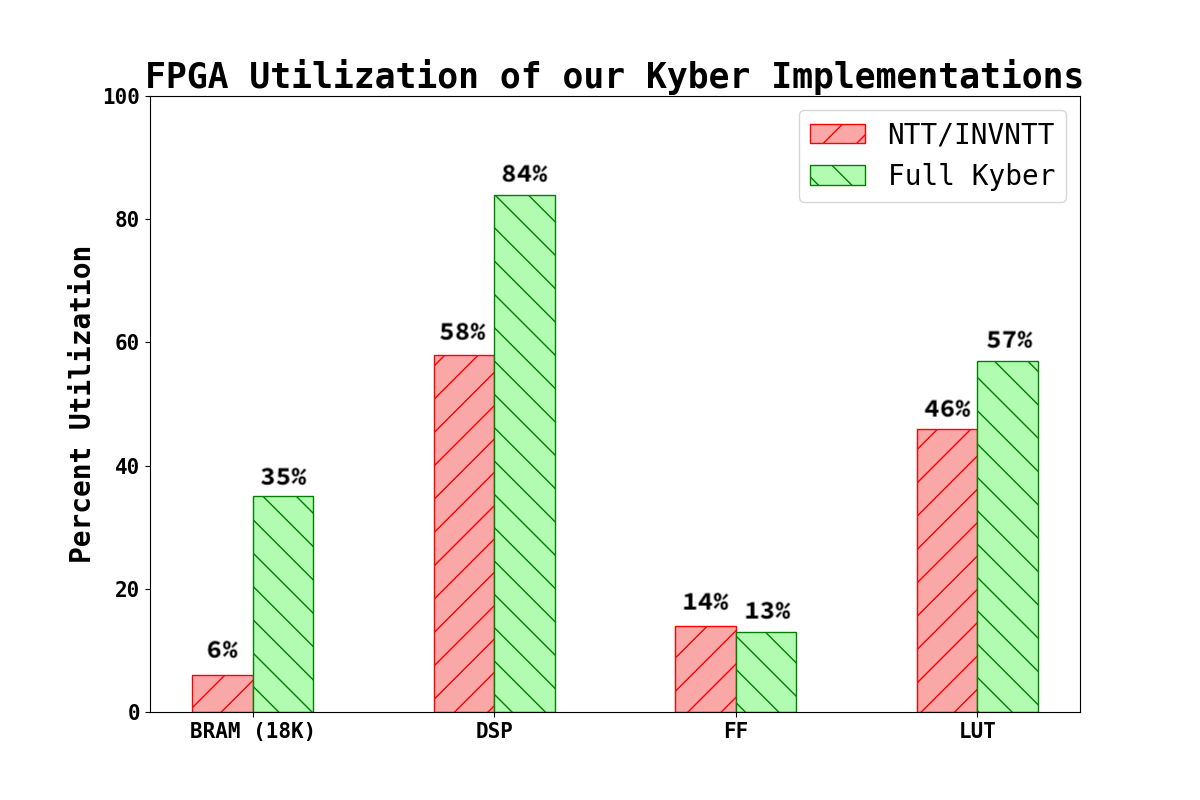
\includegraphics[width=\linewidth]{imgs/results-synth-util.png}
    \caption{The hardware utilization of the different FPGA implementations}
    \label{fig:results-synth-util}
  \end{subfigure}\hspace{0.05\textwidth}%
  \begin{subfigure}{.45\textwidth}
    \centering
    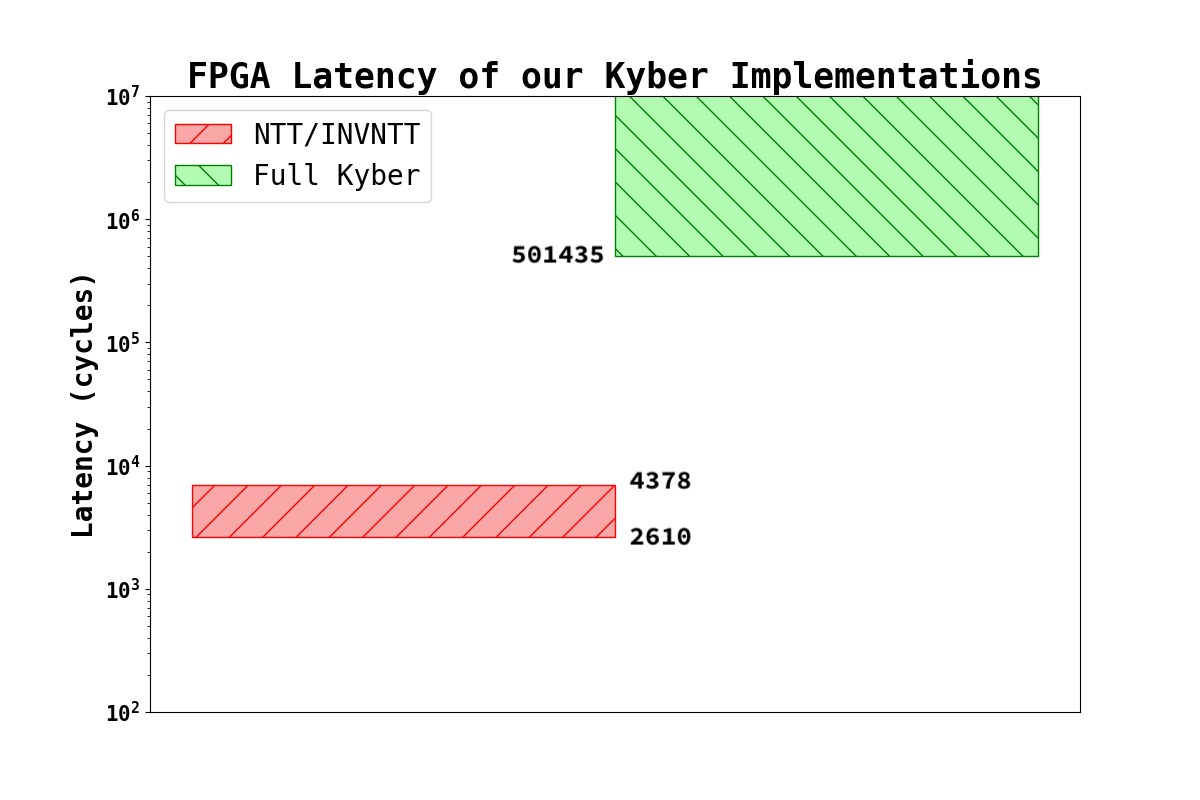
\includegraphics[width=\linewidth]{imgs/results-synth-lat.png}
    \caption{The expected latency of the different FPGA implementations}
    \label{fig:results-synth-lat}
  \end{subfigure}
  \caption{The synthesis results for our FPGA implementations}
\end{figure}

For the utilization in Figure \ref{fig:results-synth-util},
we can see that putting the entire design on FPGA hardware
results in more hardware resources overall, as expected.
One interesting note is the overall amount of DSP usage; for
both designs, a significant number are used, much more than
other labs have seen. This is due to the need for multipliers
in Montgomery conversion. Having a value in Montgomery form
can change performing a modulus over one value (as needed
for modular ring operations) to another;
by choosing to perform a modulus over a power of two, such
moduli can be implemented in hardware quickly. However,
converting in and out of this representation involves a
multiplication step. This particular operation was one of
the key reasons why the NTT kernel couldn't be as
optimized. The NTT kernel had an outer loop that required
a Montgomery conversion for each iteration, where the
number of iterations varied each time it was used. Although
we could unroll most uses of this loop, the largest version
of this loop could not be unrolled, due to the limited
number of DSP blocks available.

While the entire design used more resources in general, we
also discovered that the optimized NTT kernel surprisingly
used \textit{more} flip-flops (\code{FF}) compared to the
overall design. This seems somewhat surprising, considering
that the NTT kernels are included (multiple times) in the
entire algorithm, but makes sense once you consider the
extra optimizations applied to the NTT algorithms in
isolation. Specifically, with just the NTT algorithms, we
can exploit loop pipelining and unrolling to achieve much
higher performance by doing operations in parallel; however,
this comes at the cost of extra flip-flops to store
intermediate results in the different pipeline stages, as
well as replicated across all loop iterations. This contrasts
with the entire design in hardware; due to the lack of
available resources, we are able to optimized the design
much less, reducing the number of flip-flops needed in
this case from the lack of aggressive pipelining/unrolling.

In addition to the hardware utilization of each design, we
also compare about the predicted latency of each design;
how many cycles each design should take. For the NTT
algorithms, the latency is uncertain, as it depends on which
operation we're performing. Performing an NTT operation takes
2610 cycles, whereas performing an INVNTT operation takes 4378
cycles due to an extra multiplication reduction step needed at
the end.

% ---------------------------------------------------------
% Experimental
% ---------------------------------------------------------
% Results obtained from running the implementation on the
% FPGA

\subsection*{Experimental}

% - - - - - - - - - - - - - - - - - - - - - - - - - - - - -
% Project Management
% - - - - - - - - - - - - - - - - - - - - - - - - - - - - -

% =========================================================
% project-management.tex
% =========================================================
% A description of the project management of the team, as
% well as milestones and setbacks

\section*{Project Management}

% - - - - - - - - - - - - - - - - - - - - - - - - - - - - -
% Conclusion/Acknowledgements
% - - - - - - - - - - - - - - - - - - - - - - - - - - - - -

% =========================================================
% conclusion.tex
% =========================================================
% The conclusion of the report, including any
% acknowledgements

\section*{Conclusion}

% Note: Aidan has a pet peeve when conclusions have
% "In conclusion, ..." :)

In this project, we successfully implemented optimizations for the kyber algorithm on an FPGA. The optimization of the NTT component
demonstrated potential for significant performance improvements when optimizing a component of an algorithm. It also showcased 
the area-latency tradeoff, especially when hardware constraints of the FPGA board. The implementation of the NTT algorithms in hardware
provided some performance improvements over a pure software approach. It reduced the execution time from 120.859 ms to 105.463 ms. 
Expanding to a full hardware implementation of the kyber algorithm further reduced the execution time to 84.050 ms, which demonstrates
the potential of hardware acceleration. However, the overall speedup was constrained by several factors such as the lower clock
frequency of the FPGA compared to the ARM core and the limited hardware reuse caused by the diverse operations in the Kyber algorithm.
These results emphasize the challenges of achieving significant performance gains for complex cryptographic algorithms when there are
hardware constraints. This is relevant as FPGAs can be very useful when it comes to implementing algorithms and can be used for efficient 
implementations of post-quantum cryptographic (PQC) algorithm and it is important to continue to explore hardware accelerations of these
algorithms for the future.

% ---------------------------------------------------------
% Acknowledgements
% ---------------------------------------------------------

\subsection*{Acknowledgements}

We would like to acknowledge Professor Zhang, Yixiao Du, and Andrew Butt for their support along with all previous course staff of ECE 6775 for 
the labs, which we based some of our frameworks off of. We also acknowledge the people who developed the kyber algorithm and developed the original
github for the original reference implementation.


\newpage

% - - - - - - - - - - - - - - - - - - - - - - - - - - - - -
% References
% - - - - - - - - - - - - - - - - - - - - - - - - - - - - -

\printbibliography
\end{document}
